\documentclass{standalone}
\usepackage{graphicx}	
\usepackage{amssymb, amsmath}
\usepackage{color}

\usepackage{tikz}
\usetikzlibrary{intersections, backgrounds}

\definecolor{light}{RGB}{220, 188, 188}
\definecolor{mid}{RGB}{185, 124, 124}
\definecolor{dark}{RGB}{143, 39, 39}
\definecolor{highlight}{RGB}{180, 31, 180}
\definecolor{gray10}{gray}{0.1}
\definecolor{gray20}{gray}{0.2}
\definecolor{gray30}{gray}{0.3}
\definecolor{gray40}{gray}{0.4}
\definecolor{gray60}{gray}{0.6}
\definecolor{gray70}{gray}{0.7}
\definecolor{gray80}{gray}{0.8}
\definecolor{gray90}{gray}{0.9}
\definecolor{gray95}{gray}{0.95}

\newcommand*{\offset}{0.025}

\begin{document}

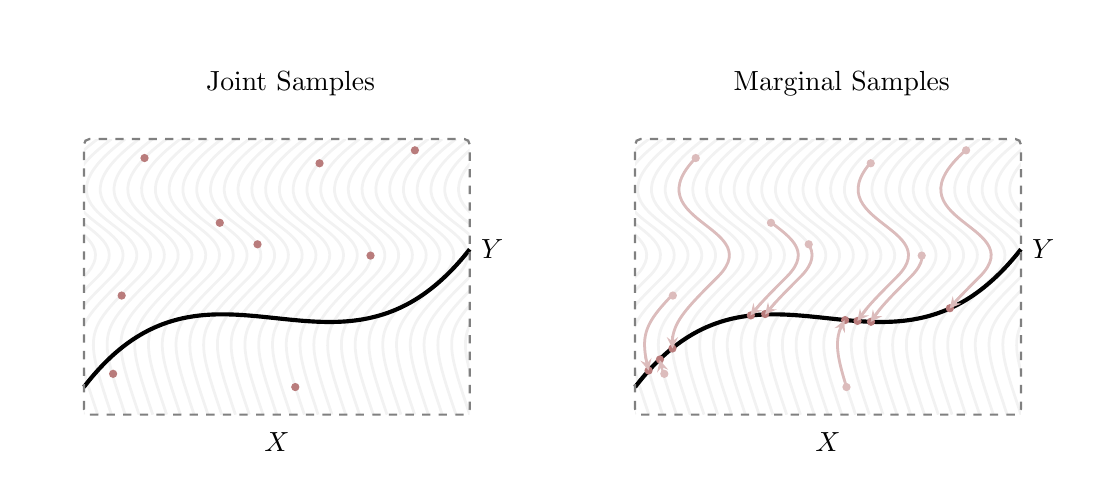
\begin{tikzpicture}[scale=0.35, thick]

\begin{scope}[shift={(0, 0)}]
  \draw[white] (3, -2) rectangle (21, 14);
  
  \node at (12.5, 12) { Joint Samples };
  
  \begin{scope}
    \clip (5, 0) rectangle +(14, 10);
    \foreach \i in {2.5, 3, ..., 21.5} {
      \draw [color=gray95, line width=1] (\i, 0) .. controls +(-1, 3) .. +(1, 5) .. 
                                         controls +(2, 2) and +(-4, -3) .. +(1, 10);
    }  
  \end{scope}
  
  \node at (12, -1) { $X$ };

  \draw [line width=1.5] (5, 1) .. controls (9.6, 7) and (14.3, 0) .. (19, 6)
  node[right] { $Y$ };
  
  \draw [rounded corners=2pt, color=gray, dashed] (5, 0) rectangle +(14, 10);
  
  \fill [fill=mid] (6.06, 1.48) circle (0.15);
  
  \fill [fill=mid] (6.37, 4.32) circle (0.15);
  
  \fill [fill=mid] (7.2, 9.31) circle (0.15);
  
  \fill [fill=mid] (9.93, 6.96) circle (0.15);
  
  \fill [fill=mid] (11.3, 6.18) circle (0.15);
  
  \fill [fill=mid] (12.67, 1) circle (0.15);
  
  \fill [fill=mid] (13.55, 9.12) circle (0.15);
  
  \fill [fill=mid] (15.4, 5.77) circle (0.15);
  
  \fill [fill=mid] (17.01, 9.59) circle (0.15);
  
\end{scope}

\begin{scope}[shift={(20, 0)}]
  \draw[white] (3, -2) rectangle (21, 14);
  
  \node at (12.5, 12) { Marginal Samples };
  
  \begin{scope}
    \clip (5, 0) rectangle +(14, 10);
    \foreach \i in {2.5, 3, ..., 21.5} {
      \draw [color=gray95, line width=1] (\i, 0) .. controls +(-1, 3) .. +(1, 5) .. 
                                         controls +(2, 2) and +(-4, -3) .. +(1, 10);
    }  
  \end{scope}
  
  %\begin{scope}
  %  \clip (5, 0) rectangle +(14, 10);
  %  \foreach \i in {6, 6.5, 7, 9.5, 10, 13, 13.5, 14, 16.5} {
  %    \draw [color=black, line width=1] (\i, 0) .. controls +(-1, 3) .. +(1, 5) .. 
  %                                       controls +(2, 2) and +(-4, -3) .. +(1, 10);
  %  }  
  %\end{scope}
  
  \node at (12, -1) { $X$ };

  \draw [line width=1.5] (5, 1) .. controls (9.6, 7) and (14.3, 0) .. (19, 6)
  node[right] { $Y$ };
  
  \draw [rounded corners=2pt, color=gray, dashed] (5, 0) rectangle +(14, 10);
  
  \begin{scope}
    \clip (5, 1.75) rectangle +(2, 2.6);
    \foreach \i in {6} {
      \draw [color=light, line width=1] (\i, 0) .. controls +(-1, 3) .. +(1, 5) .. 
                                         controls +(2, 2) and +(-4, -3) .. +(1, 10);
    }  
  \end{scope}
  \fill [fill=mid] (5.49, 1.6) circle (0.15);
  \draw[->, >=stealth, light] (5.37, 2.1) -- +(0.12, -0.5);
  \fill [fill=light] (6.37, 4.32) circle (0.15);
  
  \fill [fill=mid] (5.9, 2) circle (0.15);  
  \draw[->, >=stealth, light] (6.025, 1.48) -- +(-0.13, 0.5);
  \fill [fill=light] (6.06, 1.48) circle (0.15);

  \begin{scope}
    \clip (4, 2.6) rectangle +(6, 6.7);
    \foreach \i in {7} {
      \draw [color=light, line width=1] (\i, 0) .. controls +(-1, 3) .. +(1, 5) .. 
                                         controls +(2, 2) and +(-4, -3) .. +(1, 10);
    }  
  \end{scope}
  \fill [fill=mid] (6.354, 2.4) circle (0.15);
  \draw[->, >=stealth, light] (6.354, 2.85) -- +(0.0, -0.45);
  \fill [fill=light] (7.2, 9.31) circle (0.15);

  \begin{scope}
    \clip (8, 3.8) rectangle +(12, 3.2);
    \foreach \i in {9.5} {
      \draw [color=light, line width=1] (\i, 0) .. controls +(-1, 3) .. +(1, 5) .. 
                                         controls +(2, 2) and +(-4, -3) .. +(1, 10);
    }  
  \end{scope}  
  \fill [fill=mid] (9.2, 3.6) circle (0.15);
  \draw[->, >=stealth, light] (9.56, 4.05) -- +(-0.375, -0.45);
  \fill [fill=light] (9.93, 6.96) circle (0.15);
  
  \begin{scope}
    \clip (8, 3.8) rectangle +(12, 2.4);
    \foreach \i in {10} {
      \draw [color=light, line width=1] (\i, 0) .. controls +(-1, 3) .. +(1, 5) .. 
                                         controls +(2, 2) and +(-4, -3) .. +(1, 10);
    }  
  \end{scope}
  \fill [fill=mid] (9.72, 3.65) circle (0.15);
  \draw[->, >=stealth, light] (10.09, 4.08) -- +(-0.375, -0.45);
  \fill [fill=light] (11.3, 6.18) circle (0.15);
  
  \begin{scope}
    \clip (8, 1) rectangle +(12, 2.25);
    \foreach \i in {13} {
      \draw [color=light, line width=1] (\i, 0) .. controls +(-1, 3) .. +(1, 5) .. 
                                         controls +(2, 2) and +(-4, -3) .. +(1, 10);
    }  
  \end{scope}
  \fill [fill=mid] (12.62, 3.43) circle (0.15);
  \draw[->, >=stealth, light] (12.4, 3) -- +(0.2, 0.425);
  \fill [fill=light] (12.67, 1) circle (0.15);
  
  \begin{scope}
    \clip (8, 3.6) rectangle +(12, 5.5);
    \foreach \i in {13.5} {
      \draw [color=light, line width=1] (\i, 0) .. controls +(-1, 3) .. +(1, 5) .. 
                                         controls +(2, 2) and +(-4, -3) .. +(1, 10);
    }  
  \end{scope}
  \fill [fill=mid] (13.07, 3.4) circle (0.15);
  \draw[->, >=stealth, light] (13.42, 3.85) -- +(-0.355, -0.45);
  \fill [fill=light] (13.55, 9.12) circle (0.15);
  
  \begin{scope}
    \clip (8, 3.6) rectangle +(12, 2.3);
    \foreach \i in {14} {
      \draw [color=light, line width=1] (\i, 0) .. controls +(-1, 3) .. +(1, 5) .. 
                                         controls +(2, 2) and +(-4, -3) .. +(1, 10);
    }  
  \end{scope}
  \fill [fill=mid] (13.56, 3.37) circle (0.15);
  \draw[->, >=stealth, light] (13.88, 3.81) -- +(-0.335, -0.45);
  \fill [fill=light] (15.4, 5.77) circle (0.15);

  \begin{scope}
    \clip (8, 4.1) rectangle +(12, 5.5);
    \foreach \i in {16.5} {
      \draw [color=light, line width=1] (\i, 0) .. controls +(-1, 3) .. +(1, 5) .. 
                                         controls +(2, 2) and +(-4, -3) .. +(1, 10);
    }  
  \end{scope}  
  \fill [fill=mid] (16.42, 3.86) circle (0.15);
  \draw[->, >=stealth, light] (16.8, 4.3) -- +(-0.39, -0.45);
  \fill [fill=light] (17.01, 9.59) circle (0.15);
  
\end{scope}

\end{tikzpicture}

\end{document}  